\documentclass{article}

\usepackage{graphicx}
\usepackage{tikz}
\usepackage{tikzsymbols}
\usetikzlibrary{calc,patterns,shapes.geometric}
\pagestyle{empty}
\usepackage[margin=0pt]{geometry}
\geometry{papersize={14in,12in}}

\def\centerarc[#1](#2)(#3:#4:#5){\draw[#1] ($(#2)+({#5*cos(#3)},{#5*sin(#3)})$) arc (#3:#4:#5);}

\begin{document}
	\begin{figure}
		\centering
		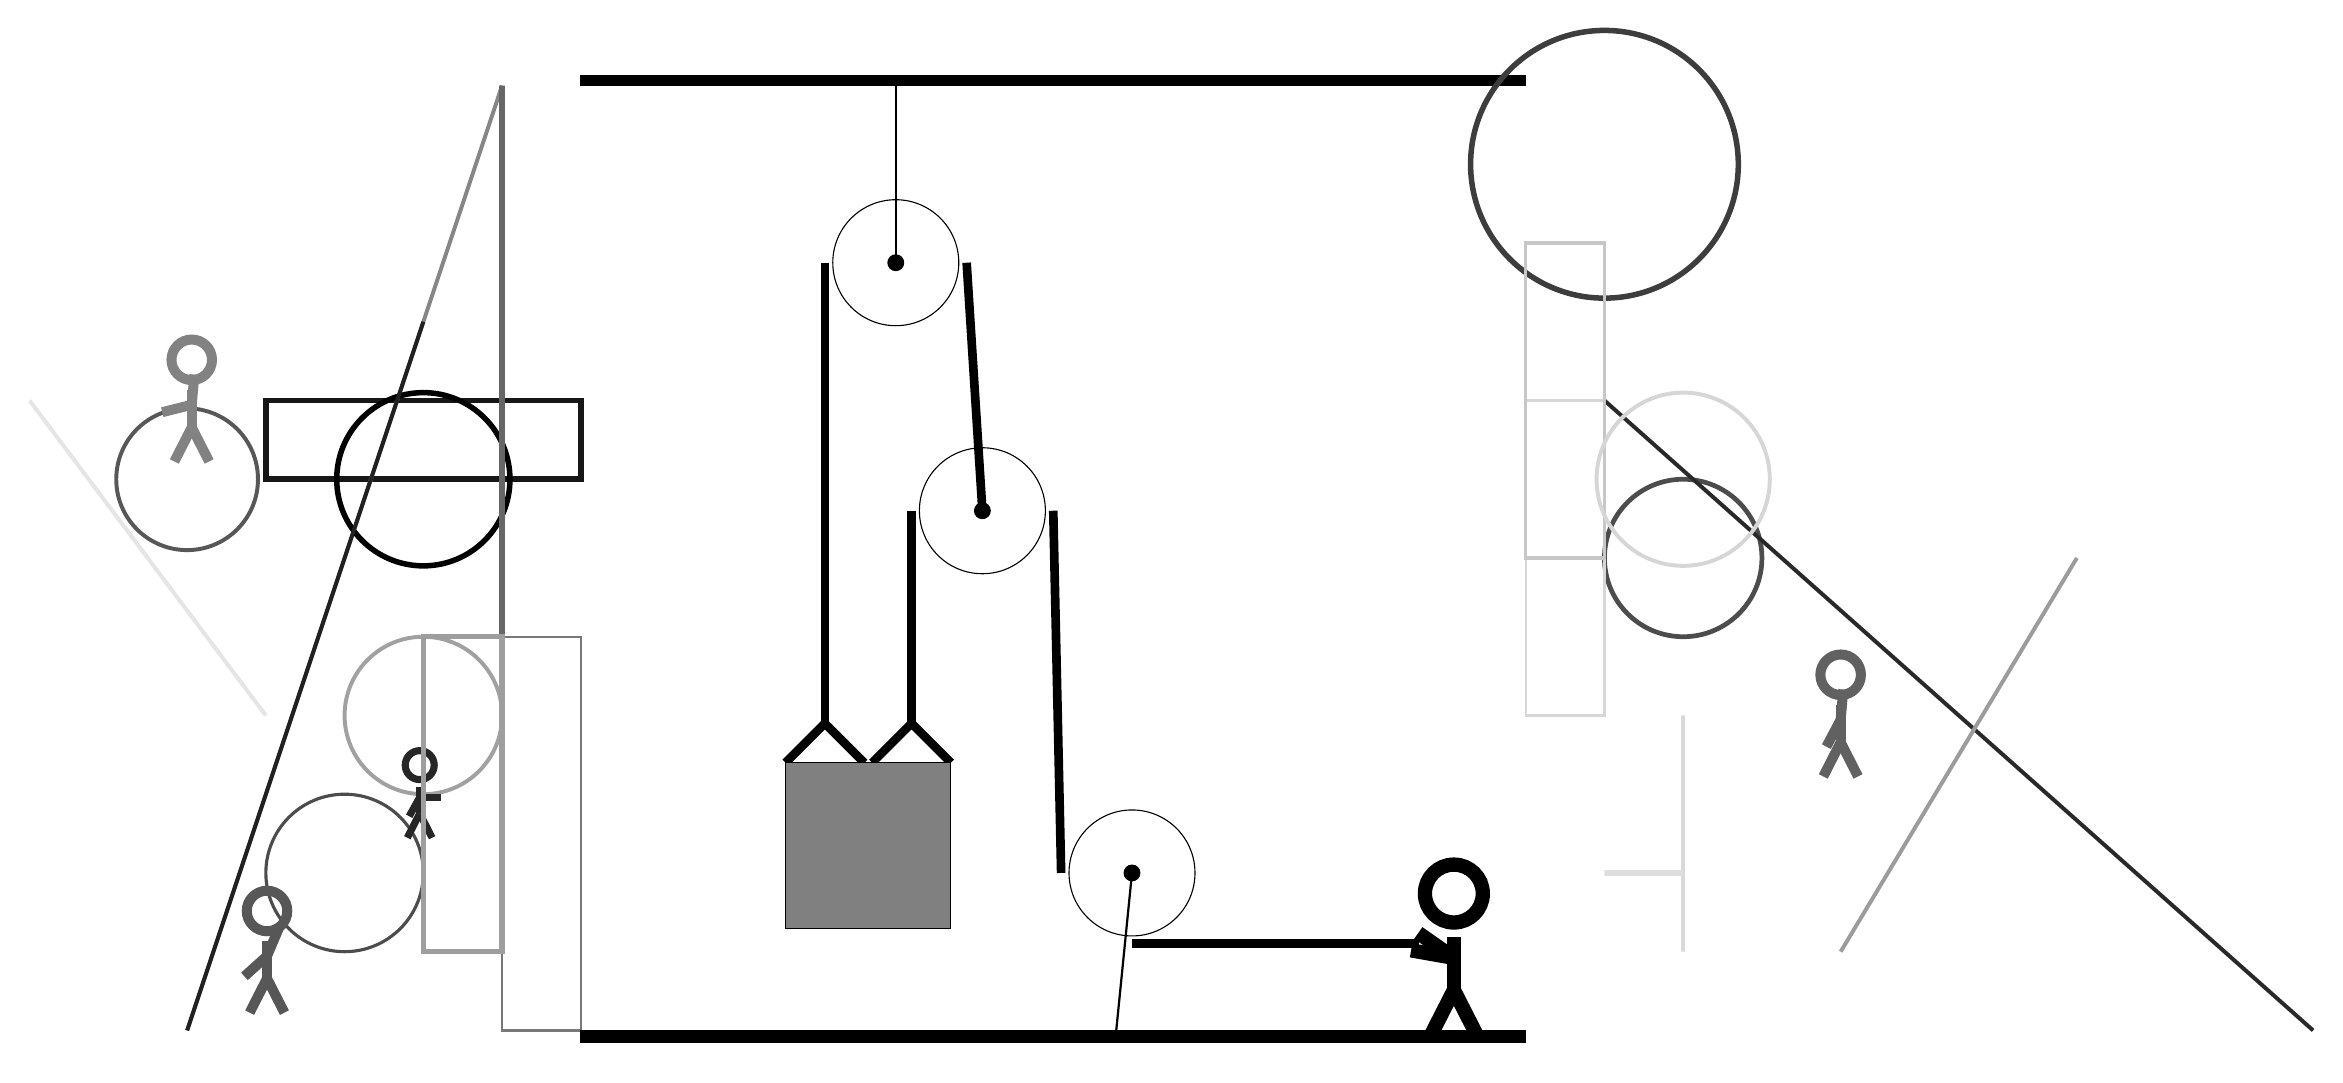
\begin{tikzpicture}
			%%%%% START %%%%%
			
			\draw[fill=black] (-2, 9) rectangle (10, 9.125);
			
			\draw (2, 6.75) circle (0.8);
			\draw[fill=black] (2, 6.75) circle (0.1);
			\draw[thick] (2, 6.75) -- (2, 9);
			
			\draw (3.1, 3.6) circle (0.8);
			\draw[fill=black] (3.1, 3.6) circle (0.1);
			
			\draw (5, -1) circle (0.8);
			\draw[fill=black] (5, -1) circle (0.1);
			\draw[thick] (5, -1) -- (4.8, -3);
			
			\draw[line width = 1.1mm]  (0.6, 0.4) -- (1.1, 0.9) -- (1.6, 0.4);
			\draw[line width = 1.1mm]  (1.7, 0.4) -- (2.2, 0.9) -- (2.7, 0.4);
			\draw[fill=black!50] (0.6, 0.4) rectangle (2.7, -1.7);
			
			\draw [line width=0.7mm, color=black!76](11, 8) circle (1.7);
			
			\draw [line width=0.5mm, color=black!66](-7, 4) circle (0.9);
			\draw [line width=0.6mm, color=black!70](12, 3) circle (1.0);
			\draw[line width=0.3mm, color=black!16] (11, 1) rectangle (10, 5);
			\draw[line width=0.3mm, color=black!53] (-3, 2) rectangle (-2, -3);
			
			\draw[line width=0.5mm, color=black!15] (12, 1) rectangle (12, -2);
			\draw[line width=0.5mm, color=black!84](11, 5) -- (20, -3);
			
			\draw[line width=0.7mm, color=black!91] (-2, 5) rectangle (-6, 4);
			\draw [line width=0.5mm, color=black!37](-4, 1) circle (1.0);
			\draw [line width=0.4mm, color=black!70](-5, -1) circle (1.0);
			\node[line width=0.4mm, color=black!85] at (-4, 0) {\Strichmaxerl[5][61][0]};
			\node[line width=0.3mm, color=black!62] at (14, 1) {\Strichmaxerl[7][62][85]};
			\draw[line width=0.5mm, color=black!47](-7, -3) -- (-3, 9);
			
			\node[line width=0.3mm, color=black!49] at (-7, 5) {\Strichmaxerl[7][14][85]};
			\draw [line width=0.7mm, color=black!100](-4, 4) circle (1.1);
			\draw[line width=0.5mm, color=black!39](14, -2) -- (17, 3);
			\draw[line width=0.5mm, color=black!87](-4, 6) -- (-7, -3);
			
			\draw[line width=0.7mm, color=black!60] (-3, -2) rectangle (-3, 9);
			\draw[line width=0.7mm, color=black!38] (-4, 2) rectangle (-3, -2);
			
			\draw[line width=0.4mm, color=black!22] (10, 7) rectangle (11, 3);
			\draw[line width=0.7mm, color=black!13] (11, -1) rectangle (12, -1);
			
			\draw [line width=0.5mm, color=black!16](12, 4) circle (1.1);
			
			\node[line width=0.2mm, color=black!66] at (-6, -2) {\Strichmaxerl[7][42][67]};
			\draw [line width=0.2mm, color=black!39](11, 0) circle (0.0);
			\draw[line width=0.5mm, color=black!10](-6, 1) -- (-9, 5);
			
			
			\draw[line width = 1.1mm] (1.1, 6.75) -- (1.1, 0.9);
			\centerarc[line width = 1.1mm](2, 6.75)(0:180:0.9);
			\draw[line width = 1.1mm] (2.9, 6.75) -- (3.1, 3.6);
			\draw[line width = 1.1mm] (2.2, 3.6) -- (2.2, 0.9);
			\centerarc[line width = 1.1mm](3.1, 3.6)(0:180:0.9);
			\draw[line width = 1.1mm] (4.0, 3.6) -- (4.1, -1);
			\centerarc[line width = 1.1mm](5, -1)(180:270:0.9);
			\draw[line width = 1.1mm] (5, -1.9) -- (8.65, -1.9);
			
			\node at (9, -2) {\Strichmaxerl[10][-35][170]};
			
			\draw[fill=black] (-2, -3) rectangle (10, -3.15);
			
			%%%%% END %%%%%
		\end{tikzpicture}
	\end{figure}	
\end{document}